\part{OO Design Basics}
\frame{\partpage}

\begin{frame}{Learning Outcomes}
	In this section you will learn how to...
	
	\begin{itemize}
		\item \textbf{Illustrate} the role of UML in communicating software design
		\item \textbf{Explain} basic OO design principles, including abstraction and polymorphism
		\item \textbf{Explain} the role of design patterns in object-orientated software design
		\item \textbf{Identify} the key components of a pattern
	\end{itemize}
\end{frame}

\begin{frame}{Object Modelling Techniques}
	\begin{itemize}
		\item Used to describe patterns in the GO4 book
		\item Uses UML to graphical represent different OO relationships:
		\begin{itemize}
			\item \textbf{class diagrams}: show the static relationship between classes
			\item \textbf{object diagrams}: show the state of a program as a series of related objects
			\item \textbf{interaction diagrams}: illustrate execution of the program as an interaction among
			related objects
		\end{itemize}
	\end{itemize}
\end{frame}

\begin{frame}{Classes}
	\begin{center}
		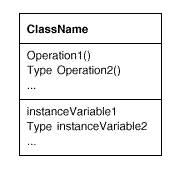
\includegraphics[width=5cm]{class_diagram.jpg}
	\end{center}
\end{frame}

\begin{frame}{Object Instantiation}
	\begin{center}
		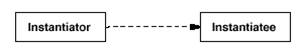
\includegraphics[width=10cm]{instance_diagram.jpg}
	\end{center}
\end{frame}

\begin{frame}{Subclassing and Abstract Classes}
	\begin{center}
		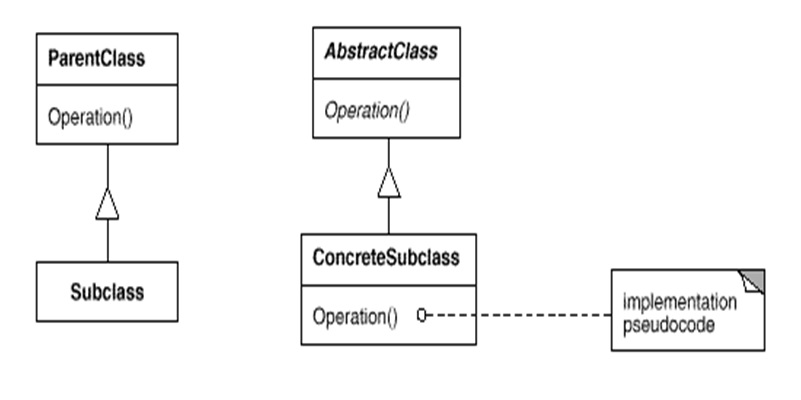
\includegraphics[width=10cm]{subclasses_and_abstraction.jpg}
	\end{center}
\end{frame}

\begin{frame}{Abstraction and Polymorphism}
	\begin{center}
		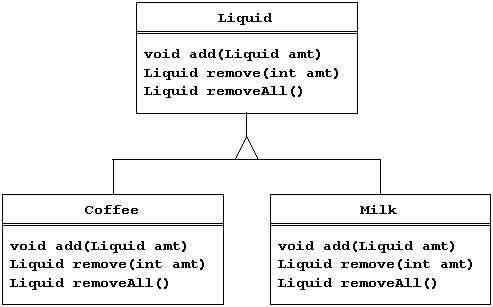
\includegraphics[width=10cm]{LiquidFamilyUML.jpg}
	\end{center}
\end{frame}

\begin{frame}{Pseudo-code and Containing}
	\begin{center}
		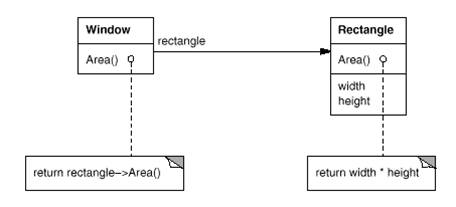
\includegraphics[width=10cm]{pseudocode_and_containment.jpg}
	\end{center}
\end{frame}

\begin{frame}{Object Diagrams}
	\begin{center}
		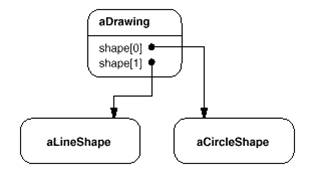
\includegraphics[width=10cm]{object_diagram.jpg}
	\end{center}
\end{frame}

\begin{frame}{Interaction Diagrams}
	\begin{center}
		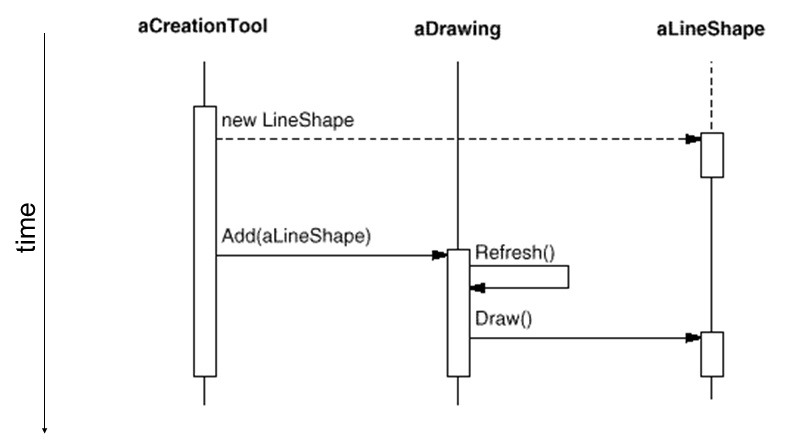
\includegraphics[width=10cm]{interaction_diagram.jpg}
	\end{center}
\end{frame}

\begin{frame}{Role of Design Patterns}
	\begin{itemize}
		\item OO design is more than just drawing diagrams, it is craftsmanship
		\item Good drafters are good designers
		\item OO design skill comes with deliberate practice and project experience
		\item A powerful form of abstraction and resuse is \textit{design} abstraction and re-use
	\end{itemize}
\end{frame}

\begin{frame}{Role of Design Patterns}
Object orientated systems tend to exhibit recurring structures that promote:

	\begin{itemize}
		\item Abstraction
		\item Flexibility
		\item Modularity
		\item Elegance
	\end{itemize}
\end{frame}

\begin{frame}{Role of Design Patterns}
	\begin{itemize}
		\item Therein lies valuable design knowledge.
		\item The challenge, of course, is to...		
		\begin{itemize}
			\item capture
			\item communicate
			\item and apply
		\end{itemize}
		\item ...this knowledge.
	\end{itemize}
\end{frame}

\begin{frame}{Role of Design Patterns}
A design pattern...

	\begin{itemize}
		\item Abstracts a recurring design structure
		\item Comprises class and/or object	
		\begin{itemize}
			\item dependencies
			\item structures
			\item interactions
			\item conventions
		\end{itemize}
		\item names and specifies the design structure explicitly
		\item and thereby distils design experience
	\end{itemize}
\end{frame}

\begin{frame}{Components of a Design Pattern}
A design pattern is comprised of:

	\begin{itemize}
		\item A name
		\item Common aliases --- \textit{also known as}...	
		\item Real-world examples
		\item Contexts
		\item Common problems solved
		\item Solution
		\item Structure
		\item Diagrams
		\item Consequences
	\end{itemize}
\end{frame}

\begin{frame}{Components of a Design Pattern}
	\begin{itemize}
		\item Design patterns are often tacit knowledge made explicit.
		\item You will develop tacit knowledge of patterns through regular design practice.
		\item You are expected to engage in constant research and reflection
		when designing software to learn all of these different patterns.
		\item They will help you communicate and design in the future.
		\item Additional research will be required as the number of patterns greatly
		exceeds those that can be covered in workshops.
	\end{itemize}
\end{frame}

\part{Design Patterns}
\frame{\partpage}

\begin{frame}{Learning Outcomes}
	In this section you will learn how to...
	
	\begin{itemize}
		\item \textbf{Distinguish} between creational, structural, and behavoral design patterns
		\item \textbf{Compare and contrast} different design patterns
		\item \textbf{Suggest} the most appropriate design pattern for a given context
	\end{itemize}
\end{frame}

\begin{frame}{Types of Design Pattern}
Design patterns come in three main flavours:

	\begin{itemize}
		\item \textbf{creational}: concerned with the process of creating and managing the creation of objects.
		\item \textbf{structural}: dealing with the composition of objects.
		\item \textbf{behavioural}: characterizing the different means by which objects can interact with others.
	\end{itemize}
\end{frame}

\begin{frame}{Types of Design Pattern}
	\begin{columns}[onlytextwidth]
		\begin{column}{0.33\textwidth}
			\begin{itemize}
				\item \textbf{Creational}
				\item Singleton
				\item Typesafe Enum
				\item Factory
				\item Prototype
				\item Builder
			\end{itemize}
		\end{column}
		\begin{column}{0.33\textwidth}
			\begin{itemize}
				\item \textbf{Structural}
				\item Adapter
				\item Bridge
				\item Proxy
				\item Facade
				\item Decorator
			\end{itemize}
		\end{column}
		\begin{column}{0.33\textwidth}
			\begin{itemize}
				\item \textbf{Behavioural}
				\item Template
				\item State
				\item Observer
				\item Visitor				
				\item Strategy
			\end{itemize}
		\end{column}
	\end{columns}
\end{frame}

\begin{frame}{Design Patterns}
	We will now briefly examine these patterns. Throughout this section...
	
	\begin{itemize}
		\item \textbf{Please} make notes on Slack
		\item \textbf{Link} to on-line resources
		\item \textbf{Ask} questions
		\item \textbf{Think} about how the patterns may apply to your own projects
		\item \textbf{Conduct} further research
	\end{itemize}
\end{frame}

\begin{frame}{Singleton}
	\begin{center}
		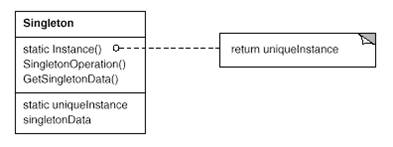
\includegraphics[width=10cm]{pattern_singleton.jpg}
	\end{center}
\end{frame}

\begin{frame}{Typesafe Enum}
	\begin{center}
		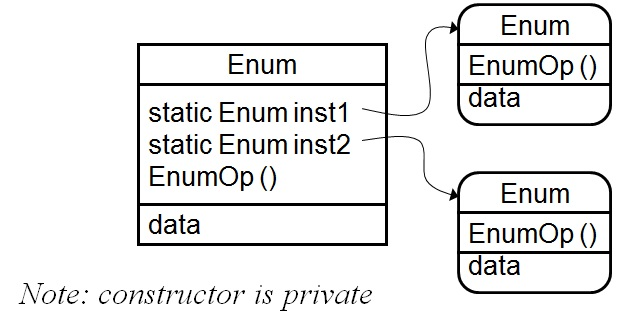
\includegraphics[width=10cm]{pattern_typesafe.jpg}
	\end{center}
\end{frame}

\begin{frame}{Abstract Factory}
	\begin{center}
		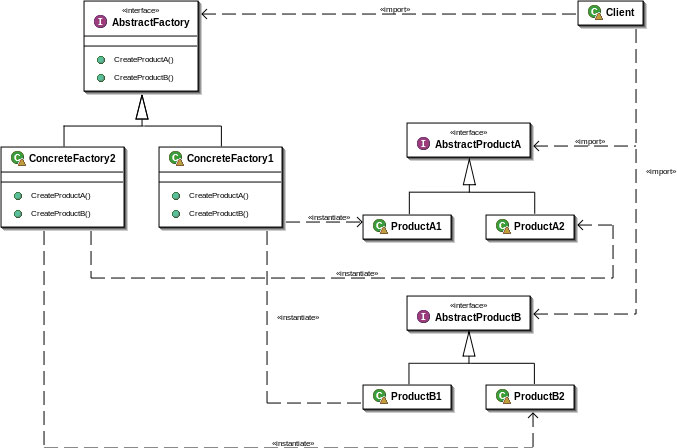
\includegraphics[width=10cm]{pattern_abstractfactory.jpg}
	\end{center}
\end{frame}

\begin{frame}{Prototype}
	\begin{center}
		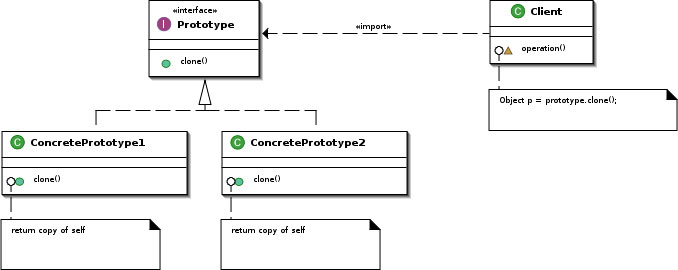
\includegraphics[width=11cm]{pattern_prototype.jpg}
	\end{center}
\end{frame}

\begin{frame}{Builder}
	\begin{center}
		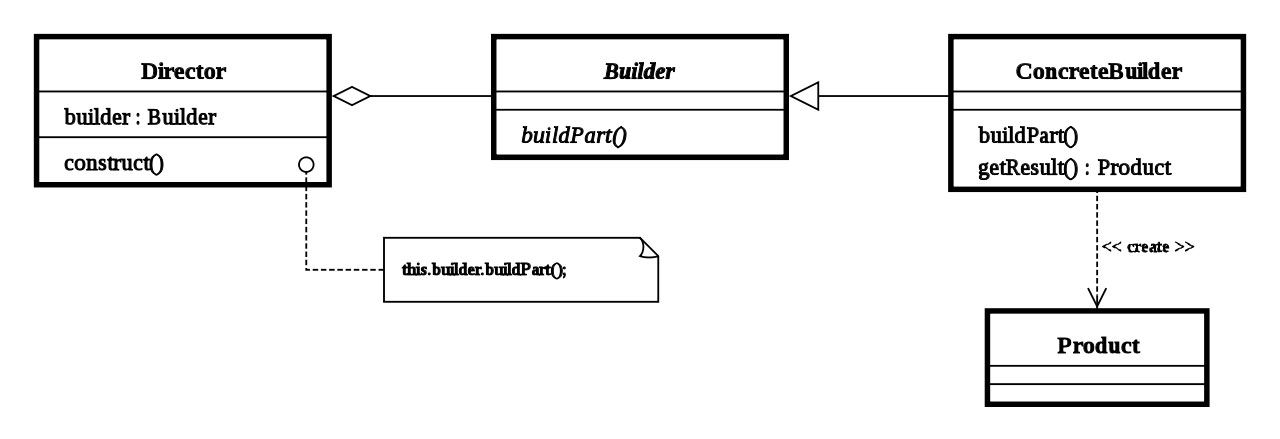
\includegraphics[width=11cm]{pattern_builder.jpg}
	\end{center}
\end{frame}

\begin{frame}{Adapter}
	\begin{center}
		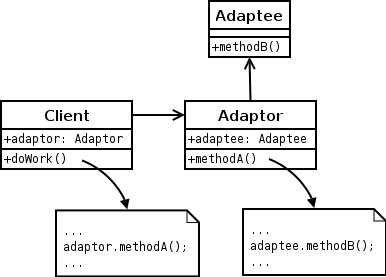
\includegraphics[width=10cm]{pattern_adapter.jpg}
	\end{center}
\end{frame}

\begin{frame}{Bridge}
	\begin{center}
		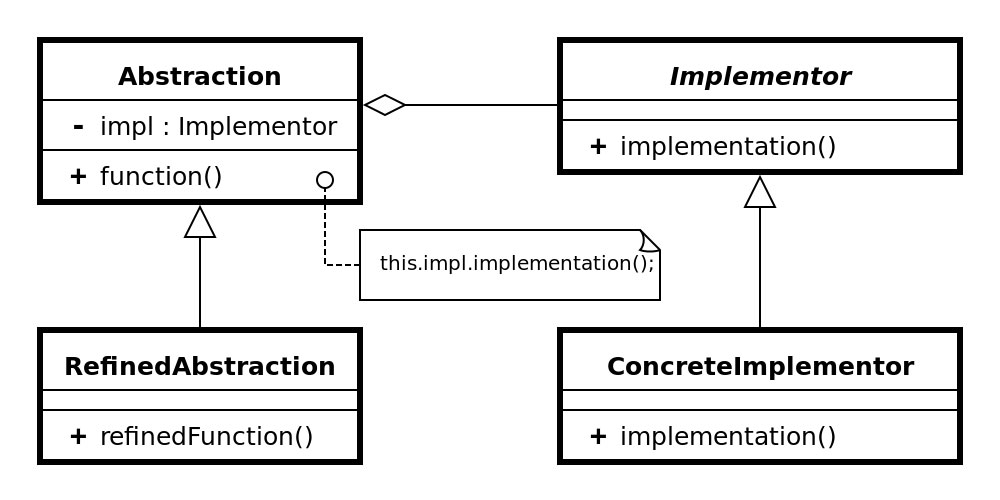
\includegraphics[width=10cm]{pattern_bridge.jpg}
	\end{center}
\end{frame}

\begin{frame}{Proxy}
	\begin{center}
		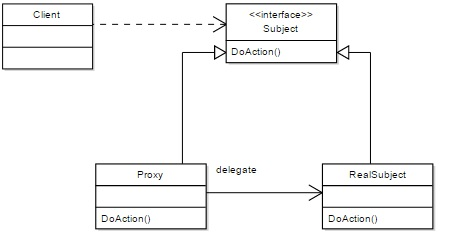
\includegraphics[width=10cm]{pattern_proxy.jpg}
	\end{center}
\end{frame}

\begin{frame}{Facade}
	\begin{center}
		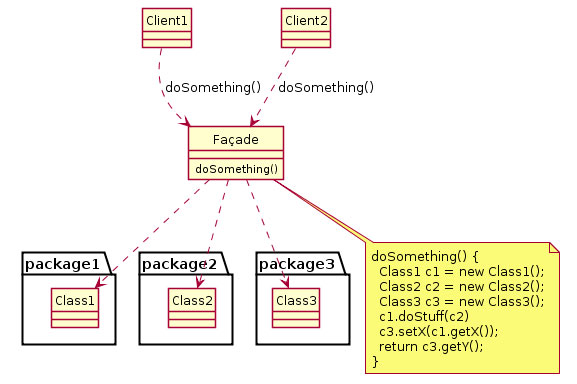
\includegraphics[width=10cm]{pattern_facade.jpg}
	\end{center}
\end{frame}

\begin{frame}{Decorator}
	\begin{center}
		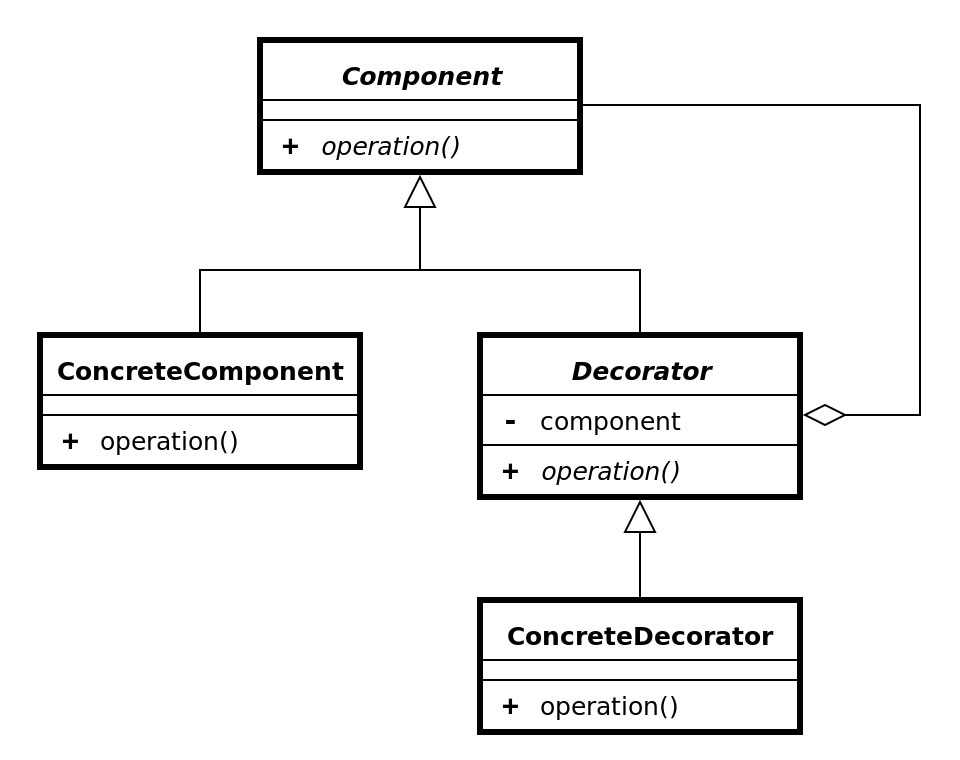
\includegraphics[width=8cm]{pattern_decorator.jpg}
	\end{center}
\end{frame}

\begin{frame}{Template}
	\begin{center}
		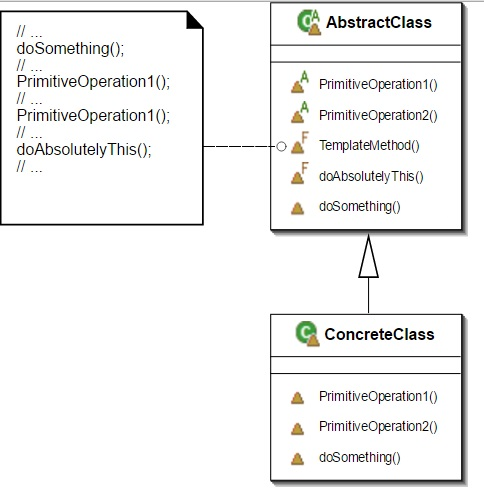
\includegraphics[width=7cm]{pattern_template.jpg}
	\end{center}
\end{frame}

\begin{frame}{State}
	\begin{center}
		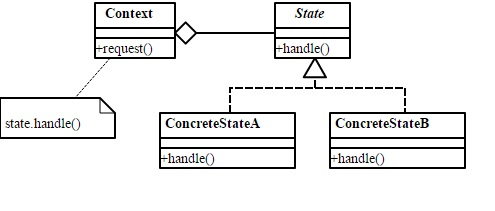
\includegraphics[width=10cm]{pattern_state.jpg}
	\end{center}
\end{frame}

\begin{frame}{Observer}
	\begin{center}
		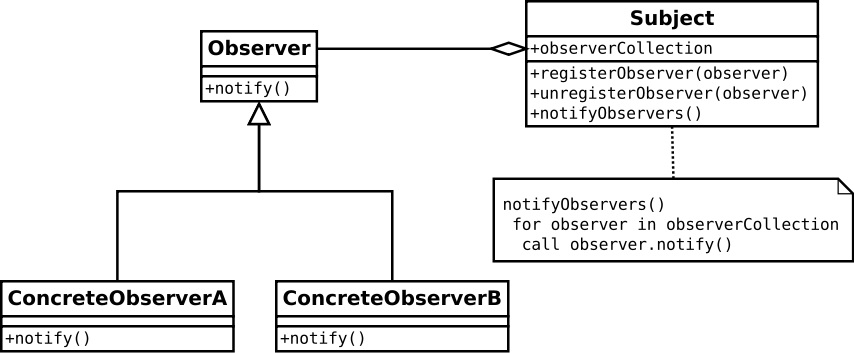
\includegraphics[width=11cm]{pattern_observer.jpg}
	\end{center}
\end{frame}

\begin{frame}{Visitor}
	\begin{center}
		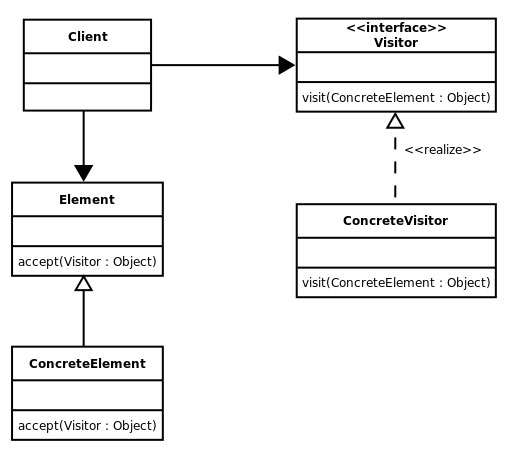
\includegraphics[width=8cm]{pattern_visitor.jpg}
	\end{center}
\end{frame}

\begin{frame}{Strategy}
	\begin{center}
		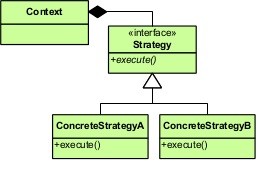
\includegraphics[width=10cm]{pattern_strategy.jpg}
	\end{center}
\end{frame}